\chapter{Wave optical simulation of the spatio-angular microscope}
\label{sec:sim-angle}
\begin{figure}[!hbt]
  \centering
  \def\svgscale{1.5}
  \input{memi-simple2.eps_tex}
  \caption{Given two masks for MMA and LCoS plane, it is possible to
    predict the light intensity in the sample by propagating fields
    from each MMA pixel into sample space and integrating an
    incoherent sum there.}
  \label{fig:memi-simple2-app}
\end{figure}
The objective of an optical microscope is defined by its support on
the Ewald sphere, i.e.\ the set of angles where $k-$vectors contribute
to the amplitude distribution $\vect E(x,y,z)$. In the following we
assume an ideal air objective with unit numerical aperture. This
objective collects all light emitted into one half space and therefore
half the Ewald sphere (\figref{fig:simple-apsf}~left).

The following code calculates the amplitude point spread function
$\vect E(x,y,z)$ of such an objective (see
\figref{fig:simple-apsf}~right for its $xz-$cross section).

{\small
\begin{verbatim}
n = 128;
nh = n/2;

% generate spherical shell in k-space
a = sinc(rr(n,n,n));
ka = ift(a);

% select top of the shell (NA=n):
ke = ka * (zz(ka)<0);

% show kx-kz section of ewald-sphere
ke(:,nh,:)

e = ift(ke);

% xz section of electric field
e(:,nh,:)
\end{verbatim}
% writeim(255/max(abs(ke(:,nh,:)))*abs(squeeze(ke(:,nh,:))),'/home/martin/thesis/kielhorn/sim-angle/ewald_xz.jpg','JPEG')
% writeim(255/max(abs(e(:,nh,:)))*abs(squeeze(e(:,nh,:))),'/home/martin/thesis/kielhorn/sim-angle/field_xz.jpg','JPEG')

\begin{figure}[!hbt]
  \centering
  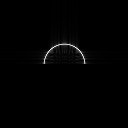
\includegraphics[width=4cm]{ewald_xz}
  \quad\quad
  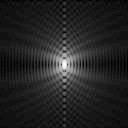
\includegraphics[width=4cm]{field_xz}
  \caption{{\bf left:} $k_xk_z-$cross section of the Ewald sphere --
    the $k-$vectors that can traverse the objective lens. {\bf right:}
    $xz-$cross section of electric field in sample space (amplitude
    point spread function).}
  \label{fig:simple-apsf}
\end{figure}

If the microscope contained no MMA but just the LCoS being illuminated
by a parallel wave, then we could obtain the 3D field distribution in the sample like this:
\begin{itemize}
\item Propagate the field from the LCoS plane into the back focal
  plane of the objective (by a single 2D Fourier transform).
\item Multiply each of the points of the Ewald sphere with the
  corresponding complex value of the illumination field.
\item 3D Fourier transform to compute the 3D field distribution within
  the sample.
\item Obtain 3D intensity distribution in sample space by computing
  the absolute square of the field.
\end{itemize}

In the case of our spatio-angular microscope each of the pixels of the
MMA can be assumed to be an independent coherent source. We think of
each of the MMA pixels as an independent mono-mode laser diode. In the
following code their fields are separately propagated into sample
space and then incoherently summed into the 3D intensity distribution.

The right picture in \figref{fig:sim-bfp-intens} displays an
$xz-$cross section of the intensity distribution for the masks shown
in in \figref{fig:mma-lcos-window}. Note that the MMA window is
shifted slightly to the right. The intensity distribution in
\figref{fig:sim-bfp-intens} right shows that some angles are missing.

\begin{verbatim}
% define rectangular window as an lcos pattern
lcx = 0;
lcy = 10;
lw = 32;
lh = 32;
lsx = lcx-lw/2;
lex = lcx+lw/2;
lsy = lcy-lh/2;
ley = lcy+lh/2;
lcos= lsx<=xx(n,n) & xx(n,n)<lex & lsy<=yy(n,n) & yy(n,n)<ley

% define a circular window as an mma image (with quite low resolution)
mmazoom = 4;
mman = n / mmazoom;
mma = (xx(mman,mman)-3)^2+(yy(mman,mman)-0)^2 < 4^2
\end{verbatim}
% writeim(255*lcos,'/home/martin/thesis/kielhorn/sim-angle/sim-lcos-window.jpg','JPEG'); writeim(255*mma,'/home/martin/thesis/kielhorn/sim-angle/sim-mma-window.jpg','JPEG')

\begin{figure}[!hbt]
  \centering
  
\includegraphics[width=4cm]{sim-mma-window}
  \quad\quad
  
\includegraphics[width=4cm]{sim-lcos-window}
  \caption{{\bf left:} circular MMA window with 45 ``on'' pixels. {\bf
      right:} Rectangular mask for LCoS.}
  \label{fig:mma-lcos-window}
\end{figure}


\begin{verbatim}
intens = newim(n,n,n);
% visit each point in the mma image
for i=0:mman-1
    for j=0:mman-1
        if mma(i,j)
            rphase=newim(n,n);
            rphase(mmazoom*i,mmazoom*j) = 1.0;
            % create corresponding illumination direction on lcos plane
            bfp=ft(lcos .* ift(rphase));
            field=ift(repmat(bfp,[1 1 n]) .* ke);
            % accumulate intensity image (incoherent)
            intens = intens+field.*conj(field);
        end
    end
end

intens(:,nh,:)
\end{verbatim}}
% writeim(255*abs(bfp)/max(abs(bfp)),'/home/martin/thesis/kielhorn/sim-angle/sim-bfp.jpg','JPEG'); writeim(255*abs(squeeze(intens(:,nh,:)))/max(abs(intens(:,nh,:))),'/home/martin/thesis/kielhorn/sim-angle/sim-intens.jpg','JPEG')
\begin{figure}[!hbt]
  \centering
  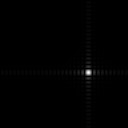
\includegraphics[width=4cm]{sim-bfp}
  \quad\quad
  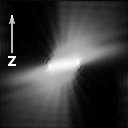
\includegraphics[width=4cm]{sim-intens}
  \caption{{\bf left:} BFP image for one particular of the ``on'' MMA
    pixels. The red circle indicates the periphery of the pupil.{\bf right:} $xz-$cross section through the intensity
    distribution in sample space.}
  \label{fig:sim-bfp-intens}
\end{figure}
